The application to be developed is a distributed one with three logic software layers: Presentation, Application and Data. The first one manages the graphical interaction with the system, the second one handles the businees logic of the application and the third one manages the storage of data involved. Thus we have a so called three-tier architecture. This architecture is a good choice to provide characteristics like scalability and maintainability mentioned in the RASD document. Each tier can be deployed in a different hardware machine (or group of machines to better achieve reliability, availability and scalability).

The mobile application communicates with the backend infrastructure directly with the application server, thus the Presentation layer is entirely contained in the app. The web application instead communicates with the Web Server, so the Presentation layer is distributed between the client and the server. 

The communication with third parties happens at the application level with synchronous messages over the Internet. To guarantee an appropiate traffic control needed to fullfill the security requirements firewalls are installed between the web server and the Internet and between the application server and the Internet. In the Data layer a backup server keeps copies of the database in order to eventually recover from faults without losses. More about the server side deployment and replication informations in the deployment section.

The following schema represents a high level logic representation of the system to be developed and deployed.

\begin{figure}[H]
    \centering
    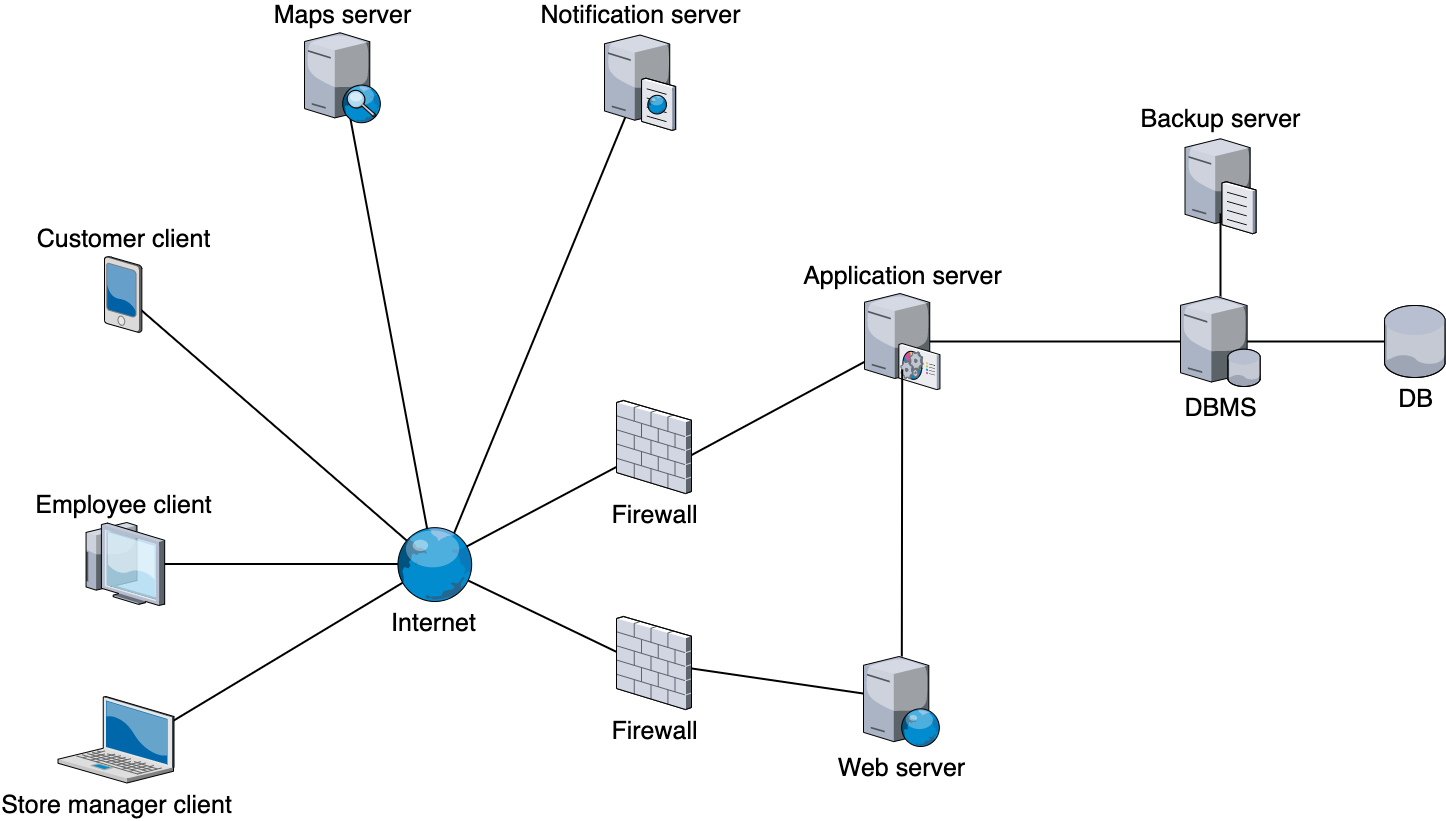
\includegraphics[width=16cm]{high_level_view.png}
\end{figure}